\documentclass[a4paper,12pt]{article}

\usepackage[utf8]{inputenc}
\usepackage[T1]{fontenc}
\usepackage{amsmath}
\usepackage{booktabs}
\usepackage{graphicx}
\usepackage{geometry}
\geometry{margin=2.5cm}
\usepackage{xcolor}
\usepackage{listings}
\usepackage{hyperref}
\hypersetup{colorlinks=true, linkcolor=blue!50!black, urlcolor=blue!50!black}
\renewcommand{\tablename}{Tabela}
\renewcommand{\figurename}{Figura}
\renewcommand{\lstlistingname}{Código}

% ---------- Configuração do realce de sintaxe (C) ----------
\definecolor{codebg}{RGB}{247,247,247}
\definecolor{codekw}{RGB}{0,0,180}
\definecolor{codecomment}{RGB}{0,128,0}
\definecolor{codestring}{RGB}{163,21,21}
\definecolor{framecolor}{RGB}{200,200,200}

\lstdefinestyle{cstyle}{
    language=C,
    backgroundcolor=\color{codebg},
    basicstyle=\ttfamily\footnotesize,
    keywordstyle=\color{codekw}\bfseries,
    commentstyle=\color{codecomment}\itshape,
    stringstyle=\color{codestring},
    numberstyle=\tiny\color{gray},
    numbers=left,
    numbersep=6pt,
    frame=single,
    rulecolor=\color{framecolor},
    breaklines=true,
    breakatwhitespace=false,
    showstringspaces=false,
    tabsize=4,
    captionpos=b,
    columns=flexible,
    morekeywords={size_t},
    extendedchars=true,
    literate=
        {á}{{\'a}}1 {à}{{\`a}}1 {â}{{\^a}}1 {ã}{{\~a}}1
        {é}{{\'e}}1 {ê}{{\^e}}1 {í}{{\'i}}1
        {ó}{{\'o}}1 {ô}{{\^o}}1 {õ}{{\~o}}1
        {ú}{{\'u}}1 {ü}{{\"u}}1 {ç}{{\c c}}1
        {Á}{{\'A}}1 {À}{{\`A}}1 {Â}{{\^A}}1 {Ã}{{\~A}}1
        {É}{{\'E}}1 {Ê}{{\^E}}1 {Í}{{\'I}}1
        {Ó}{{\'O}}1 {Ô}{{\^O}}1 {Õ}{{\~O}}1
        {Ú}{{\'U}}1 {Ü}{{\"U}}1 {Ç}{{\c C}}1
}

\title{Tarefa 16: Implementação de Produto Matriz-Vetor Usando MPI}
\author{Israel Soares de Castro Filho \\ Matrícula: 20250070780}
\date{}

\begin{document}

\maketitle

\section{Introdução}

A tarefa consiste em calcular $y = A\,x$, com $A$ de tamanho $M \times N$ e $x$ de tamanho $N$, usando MPI. A matriz é dividida por linhas com \texttt{MPI\_Scatter}, o vetor $x$ é enviado inteiro a todos com \texttt{MPI\_Bcast}, e o resultado é reunido no processo 0 com \texttt{MPI\_Gather}.

O objetivo é comparar os tempos para diferentes tamanhos de matriz e números de processos, e entender \textbf{quanto do tempo é gasto em comunicação}, principalmente no \texttt{Scatter} e no \texttt{Bcast}.

\section{Metodologia}

\paragraph{Ambiente.} Código em C com MPI (Open MPI), executado no supercomputador NPAD, partição \texttt{amd-512}, em 2 nós alocados de forma exclusiva e submetido via SLURM.

\paragraph{Estratégia.}
\begin{itemize}
    \item O processo 0 cria $A$ e $x$ (valores determinísticos).
    \item \texttt{MPI\_Scatter}: cada processo recebe $M/P$ linhas de $A$.
    \item \texttt{MPI\_Bcast}: todos recebem uma cópia completa de $x$.
    \item Cada processo calcula suas linhas de $y$; o \texttt{MPI\_Gather} leva tudo ao processo 0.
\end{itemize}

\paragraph{Como as operações coletivas funcionam (visão geral).}
\begin{itemize}
    \item \textbf{\texttt{MPI\_Scatter}}: um processo (o \textit{root}) divide um buffer em $P$ blocos iguais e entrega o bloco $i$ ao processo $i$. Todos os dados de $A$ \emph{saem de um único processo}, então o volume que o root precisa mover é aproximadamente o tamanho de $A$ inteiro, independente de $P$. O root também copia o seu próprio bloco para o buffer local.
    \item \textbf{\texttt{MPI\_Bcast}}: o root envia o \emph{mesmo} dado a todos. As implementações costumam usar uma árvore (por exemplo, binomial): quem já recebeu ajuda a repassar, de modo que são necessárias cerca de $\log_2 P$ etapas, e não $P-1$ envios do root.
    \item \textbf{\texttt{MPI\_Gather}}: operação inversa do \texttt{Scatter}; aqui só trafegam $M$ valores de $y$.
\end{itemize}

\paragraph{Volume de dados.} O que muda entre as operações é o \emph{volume}, não o número de chamadas (Tabela~\ref{tab:vol}). $A$ ocupa $8MN$ bytes, enquanto $x$ e $y$ ocupam apenas $8N$ e $8M$ bytes: $A$ é $N$ vezes maior que $x$.

\begin{table}[h!]
\centering
\begin{tabular}{rrrr}
\toprule
$M=N$ & $A$ (\texttt{Scatter}) & $x$ (\texttt{Bcast}) & $y$ (\texttt{Gather}) \\
\midrule
1024  & 8{,}4 MB  & 8{,}2 kB   & 8{,}2 kB \\
4096  & 134 MB    & 32{,}8 kB  & 32{,}8 kB \\
8192  & 537 MB    & 65{,}5 kB  & 65{,}5 kB \\
16384 & 2147 MB   & 131 kB     & 131 kB \\
\bottomrule
\end{tabular}
\caption{Volume de dados de cada operação coletiva (com $M=N$).}
\label{tab:vol}
\end{table}

\paragraph{Medição.} Cada configuração foi repetida 5 vezes (média; em cada repetição vale o processo mais lento). Foram medidos:
\begin{itemize}
    \item \textbf{tempo total}: \texttt{Scatter} + \texttt{Bcast} + cálculo + \texttt{Gather};
    \item \textbf{tempo de cálculo}: apenas o laço de multiplicação;
    \item \textbf{comunicação} = total $-$ cálculo. Inclui \texttt{Scatter}, \texttt{Bcast}, \texttt{Gather} e esperas entre processos.
\end{itemize}

\paragraph{Casos.} Intra-nó: 1, 2, 4 e 8 processos em um único nó. Inter-nó: 2, 4, 8 e 16 processos distribuídos em 2 nós, metade em cada um. Tamanhos ($M=N$): 1024, 2048, 4096, 8192 e 16384.

\section{Resultados}

A Tabela~\ref{tab:total} mostra o tempo total, e a Tabela~\ref{tab:det} detalha o maior caso. A Figura~\ref{fig:tempos} separa cálculo e comunicação para o menor e o maior tamanho.

\begin{table}[h!]
\centering
\begin{tabular}{lrrrrr}
\toprule
 & \multicolumn{5}{c}{Tempo total (ms), $M=N$} \\
\cmidrule(l){2-6}
Caso & 1024 & 2048 & 4096 & 8192 & 16384 \\
\midrule
intra, 1 proc  & 1,57 & 6,66 & 29,39 & 116,37 & 466,86 \\
intra, 2 proc  & 4,50 & 8,25 & 28,17 & 103,68 & 351,47 \\
intra, 4 proc  & 2,71 & 7,98 & 20,94 & 78,28 & 323,03 \\
intra, 8 proc  & 2,38 & 8,09 & 19,42 & 71,40 & 302,23 \\
inter, 2 proc  & 1,49 & 5,24 & 21,41 & 85,46 & 345,15 \\
inter, 4 proc  & 4,32 & 11,26 & 23,41 & 84,71 & 312,44 \\
inter, 8 proc  & 12,23 & 15,66 & 32,28 & 80,39 & 290,38 \\
inter, 16 proc & 5,74 & 8,10 & 15,14 & 42,53 & 130,99 \\
\bottomrule
\end{tabular}
\caption{Tempo total em milissegundos.}
\label{tab:total}
\end{table}

\begin{table}[h!]
\centering
\small
\begin{tabular}{lrrrrrr}
\toprule
Caso ($M=N=16384$) & Total & Cálculo & Comun. & Comun. & Speedup & Speedup \\
 & (ms) & (ms) & (ms) & (\%) & total & cálculo \\
\midrule
intra, 1 proc  & 466,9 & 269,0 & 197,9 & 42\% & 1,00 & 1,00 \\
intra, 2 proc  & 351,5 & 135,8 & 215,7 & 61\% & 1,33 & 1,98 \\
intra, 4 proc  & 323,0 & 68,7  & 254,3 & 79\% & 1,45 & 3,91 \\
intra, 8 proc  & 302,2 & 34,8  & 267,4 & 88\% & 1,54 & 7,73 \\
inter, 2 proc  & 345,1 & 135,6 & 209,6 & 61\% & 1,35 & 1,98 \\
inter, 4 proc  & 312,4 & 70,1  & 242,4 & 78\% & 1,49 & 3,84 \\
inter, 8 proc  & 290,4 & 34,4  & 256,0 & 88\% & 1,61 & 7,82 \\
inter, 16 proc & 131,0 & 17,9  & 113,1 & 86\% & 3,56 & 15,00 \\
\bottomrule
\end{tabular}
\caption{Detalhamento para $M=N=16384$. Speedup em relação a 1 processo.}
\label{tab:det}
\end{table}

\begin{figure}[h!]
\centering
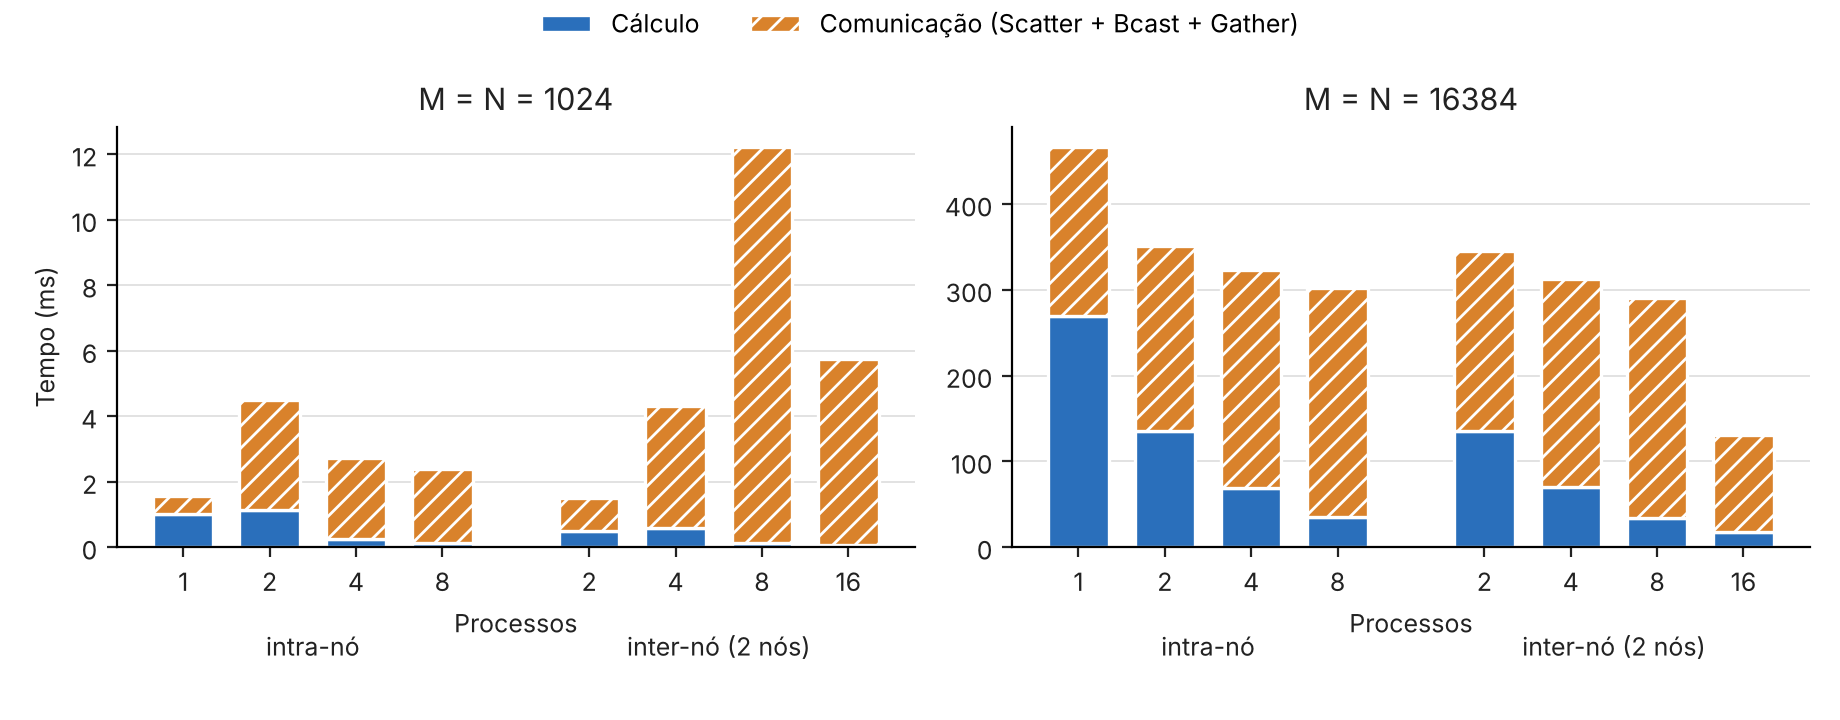
\includegraphics[width=\textwidth]{../dados/tempos.png}
\caption{Tempo dividido entre cálculo e comunicação para $M=N=1024$ e $M=N=16384$.}
\label{fig:tempos}
\end{figure}

\section{Análise}

\paragraph{O cálculo escala bem, o tempo total não.} Para $16384$, o speedup do cálculo é quase ideal (7,7 com 8 processos e 15,0 com 16), mas o do tempo total fica em apenas 1,5 com 8 processos no mesmo nó. A causa é a comunicação, que passa de 42\% do tempo com 1 processo para 88\% com 8.

\paragraph{Impacto do \texttt{MPI\_Scatter}.} É a operação dominante. Ela move $A$ inteira (2,1~GB) a partir de um único processo, então o custo é limitado pela capacidade do root de copiar e enviar dados. Aumentar $P$ divide o cálculo, mas \emph{não reduz o volume que o root precisa distribuir}; por isso a comunicação ficou na faixa de 200 a 270~ms para 1 a 8 processos, e até cresceu levemente. Com 1 processo ela ainda custa 198~ms, o que é coerente com o root copiar $A$ para o buffer local, mesmo sem outro processo para receber.

\paragraph{Impacto do \texttt{MPI\_Bcast}.} Em tamanhos grandes é desprezível: $x$ tem 131~kB, cerca de 16\,000 vezes menos dado que $A$. Como o \texttt{Bcast} usa uma árvore com $\log_2 P$ etapas (1, 2, 3 e 4 etapas para $P=2,4,8,16$), seu custo cresce devagar com $P$. Em tamanhos pequenos o quadro muda: para $1024$ todos os volumes são pequenos, e o tempo passa a ser dominado pela \emph{latência} e pela sincronização das coletivas (comunicação de 87\% a 99\% do tempo nos casos com 4 ou mais processos). Nesse regime, adicionar processos \emph{piora} o tempo total (por exemplo, 12,2~ms com 8 processos em 2 nós, contra 1,6~ms com 1 processo). O valor de 12,2~ms foge do padrão (16 processos deu 5,7~ms) e pode envolver ruído ou custos de inicialização da comunicação entre nós, já que a média tem só 5 repetições.

\paragraph{Intra-nó contra inter-nó.} Com a mesma quantidade de processos, os tempos foram parecidos (por exemplo, 302~ms contra 290~ms com 8 processos em $16384$), então a rede não foi um gargalo adicional visível para esses volumes. O destaque é \texttt{inter-nó} com 16 processos: o total caiu para 131~ms (speedup 3,56) e a comunicação para 113~ms, contra cerca de 267~ms com 8 processos em um nó.

\section{Conclusão}

\begin{itemize}
    \item O ganho em tempo total é limitado pelo \texttt{MPI\_Scatter} de $A$: o volume que um único processo distribui não diminui com mais processos, enquanto o cálculo diminui quase proporcionalmente.
    \item O \texttt{MPI\_Bcast} de $x$ é barato para matrizes grandes (pouco dado, custo em árvore $\sim\log_2 P$), mas a latência das coletivas domina para matrizes pequenas, onde usar mais processos pode piorar o tempo.
    \item A paralelização compensa para matrizes grandes e, mesmo assim, de forma parcial. O melhor resultado foi 3,56 vezes mais rápido com 16 processos em 2 nós ($M=N=16384$).
    \item Como melhoria, evitar o \texttt{Scatter} gerando cada bloco de $A$ diretamente em cada processo (cada um inicializa suas linhas) eliminaria a maior parte da comunicação.
\end{itemize}

\newpage
\appendix

\section{Código-Fonte}

\lstinputlisting[style=cstyle, caption={Produto matriz-vetor com MPI (\texttt{tarefa16.c}).}, label={cod:matvec}]{../src/tarefa16.c}

\end{document}